% ------------------------------------------------------------------------------
% The implemtations shows specifically how your research was conducted.
% All the impementation details and practical tests can be listed.
% ------------------------------------------------------------------------------

\opt{never}{\addbibresource{03-tail/bibliography.bib}} % to make citation found in most IDE

\chapter{Implementation}
\label{chap:implementation}

% -- Your text goes here --
The implementation sets out the concrete realisation of the reference architecture, detailing the tools used to automate the deployment of the \gls{cloud_infrastructure} and the integration of the embedded systems. Particular attention is paid to the in-depth description of the automated pipeline. The various applications that accompany this architecture are also highlighted.

\minitoc
\newpage

% ------------------------------------------------------------------------------
\section{Reference architecture}

% -- Your text goes here --
\subsection{\Gls{cloud_infrastructure}}
An \acrfull{iac} tool was selected to orchestrate the efficient deployment of the \gls{cloud_infrastructure} on \gls{aws}, and Pulumi was chosen because of its choice of programming language, in this case Python. The use of the same programming language for the implementation of applications and the description of \gls{aws} resources provides consistency within the project.

Integrating Pulumi is simple. The resources required are described in Python files. The deployment is managed by the Pulumi \acrshort{cli}, which records the state of the infrastructure in an Amazon S3 compartment. This compartment is located in the same \gls{aws} account as the infrastructure, using Amazon S3 to store the state rather than the default Pulumi \Gls{cloud} platform, thus eliminating external dependencies. Figure \ref{fig:pulumi_overview} shows an overview of this part of the implementation.
\begin{center}
    \begingroup
    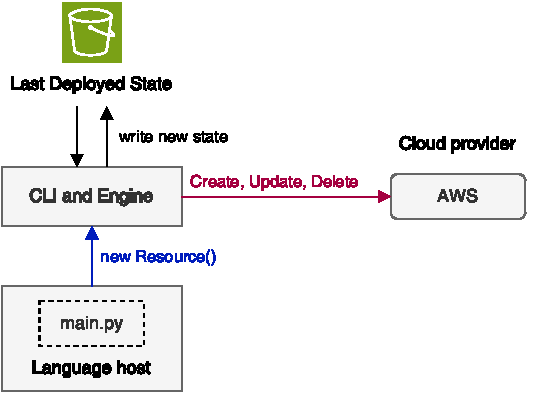
\includegraphics[width=.7\columnwidth]{implementation/pulumi_overview.pdf}
    \captionof{figure}{Overview of Pulumi's integration into the reference architecture}
    \label{fig:pulumi_overview}
    \endgroup
\end{center}
This \gls{cloud_infrastructure} part is implemented in a specific folder as follows :
\begin{center}
    \usemintedstyle{pastie}
    \begin{minted}
    [
    fontsize=\scriptsize
    ]{text}
    cloud-infrastructure
        ├── Pulumi.yaml
        ├── Pulumi.dev.yaml
        ├── Pulumi.prod.yaml
        ├── main.py
        ├── iam.py
        └── requirements.txt
    \end{minted}
\end{center}
The main configuration file for the Pulumi tool, \textit{Pulumi.yaml}, includes crucial information such as the name of the stack and the programming language used, in this case Python.

This implementation aims to facilitate the deployment of two distinct infrastructures, namely the development environment and the production environment. Therefore, two additional configuration files, \textit{Pulumi.dev.yaml} and \textit{Pulumi.prod.yaml}, are present to differentiate these two environments. \textit{Pulumi.dev.yaml} contains parameters such as the development account ID and the deployment region, while \textit{Pulumi.prod.yaml} includes the same parameters with production-specific values. The identifiers of the \gls{aws} accounts must be different.

The Python files \textit{main.py} and \textit{iam.py} detail the description of the resources to be deployed. \textit{iam.py} focuses on IAM roles and policies, while \textit{main.py} mainly covers resources related to \acrshort{iot} and other resources.

Finally, the \textit{requirements.txt} file lists the Pulumi libraries to be installed, including the main Pulumi library, which is essential for all \acrshort{iac} projects.

In terms of the Pulumi libraries used, \gls{aws} Native, a new preview, uses the \gls{aws} \Gls{cloud} Control API to manage and provision \gls{aws} resources, generally aligning with the latest \gls{aws} features as they are released. The resources available in this library are based on those defined in the \gls{aws} CloudFormation registry. In addition, \gls{aws} Classic is another library that is used to fill in resources that are not yet available in \gls{aws} Native. This library uses the \gls{aws} SDK to manage and provision these resources.


\subsection{Embedded system integration}